%%%%%%%%%%%%%%%%%%%%%%%%%%%%%%%%%%%%%%%%%%%%%%%%%%%%%%%%%%%%%%%%%%%%%%%%
%                                                                      %
%     File: PMSM_model.tex                                             %
%     Tex Master: Thesis.tex                                           %
%                                                                      %
%     Author: Israel Sother                                            %
%     Last modified: 27 May 2024                                       %
%                                                                      %
%%%%%%%%%%%%%%%%%%%%%%%%%%%%%%%%%%%%%%%%%%%%%%%%%%%%%%%%%%%%%%%%%%%%%%%%
\vfill
\section{PMSM model}\label{section:PMSM model}
As the proposed work is to improve the dynamic response and efficiency of the motor and motor drive currently used by \gls{fst}, it is necessary to first develop a model to represent this machine, a \gls{pmsm} with delta-arranged windings.

%%%%%%%%%%%%%%%%%%%%%%%%%%%%%%%%%%%%%%%%%%%%%%%%%%
\subsection{PMSM in ABC coordinates}
The stator voltages of the considered electrical machine can be given by \Cref{eq:flx_voltage_balance}, with a graphical representation in \Cref{fig:delta_model}.
\begin{equation}
	\begin{aligned}
		\begin{bmatrix}
			u_{AB} \\
			u_{BC} \\
			u_{CA} \\
		\end{bmatrix}
		=
		\begin{bmatrix}
			r_a & 0   & 0   \\
			0   & r_b & 0   \\
			0   & 0   & r_c \\
		\end{bmatrix}
		\begin{bmatrix}
			i_a \\
			i_b \\
			i_c \\
		\end{bmatrix}
		+
		\frac{d}{dt}
		\begin{bmatrix}
			\psi_a \\
			\psi_b \\
			\psi_c \\
		\end{bmatrix}
	\end{aligned}
	\label{eq:flx_voltage_balance}%chktex 24
\end{equation}

In this equation, $u_{xy}$ represents the measured voltage between terminal $x$ and $y$, $i_x$ is the current flowing on each phase, $r_x$ is the phase resistance, and $\psi_x$ is the flux linkage of each coil. Combining this in a matrix representation we can define the variables in \Cref{eq:variables_abc}.

\vspace{0.5cm}
\begin{subequations}
	\noindent\begin{minipage}{.38\linewidth}
		\begin{equation}
			\mathbf{R_{abc}} = \begin{bmatrix}
				r_a & 0   & 0   \\
				0   & r_b & 0   \\
				0   & 0   & r_c \\
			\end{bmatrix}
		\end{equation}
	\end{minipage}%
	\begin{minipage}{.3\linewidth}
		\begin{equation}
			\mathbf{i_{abc}} = \begin{bmatrix}
				i_a \\
				i_b \\
				i_c \\
			\end{bmatrix}
		\end{equation}
	\end{minipage}%
	\begin{minipage}{.3\linewidth}
		\begin{equation}
			\mathbf{u_{abc}} = \begin{bmatrix}
				u_{AB} \\
				u_{BC} \\
				u_{CA} \\
			\end{bmatrix}
		\end{equation}
	\end{minipage}%
	\label{eq:variables_abc}
\end{subequations}
\vspace{0.5cm}

Regarding the flux linkage, it can be defined as in \Cref{eq:flux_linkage}, where $\psi_{PM}$ is the permanent magnet flux linkage, and $\theta_e$ is the rotor electrical position. Additionally, the $L_{abc}$ matrix is the inductance matrix as later defined in \Cref{eq:phase_inductances}. With this definition, the \Cref{eq:flx_voltage_balance} can be expanded into \Cref{eq:voltage_balance}, where $E_x$ is the back EMF as defined in \Cref{eq:back_emf}.

\begin{subequations}
	\noindent\begin{minipage}{.5\linewidth}
		\begin{equation}
			\pmb{\psi_{abc}} = \mathbf{L_{abc}i_{abc}} + \psi_{PM} \begin{bmatrix}
				\cos{\left(\theta_e\right)} \\
				\cos{\left(\theta_e - \frac{4\pi}{3}\right)} \\
				\cos{\left(\theta_e + \frac{4\pi}{3}\right)} \\
			\end{bmatrix}
			\label{eq:flux_linkage}
		\end{equation}
	\end{minipage}%
	\begin{minipage}{.49\linewidth}
		\begin{equation}
			\mathbf{E_{abc}} = 
			\begin{bmatrix}
				E_a \\
				E_b \\
				E_c \\
			\end{bmatrix} = \psi_{PM} \dot{\theta_e}
			 \begin{bmatrix}
				-\sin{\left(\theta_e\right)} \\
				-\sin{\left(\theta_e - \frac{4\pi}{3}\right)} \\
				-\sin{\left(\theta_e + \frac{4\pi}{3}\right)} \\
			\end{bmatrix}
			\label{eq:back_emf}
		\end{equation}
	\end{minipage}%
\end{subequations}



\begin{figure}[!htb]
	\centering
	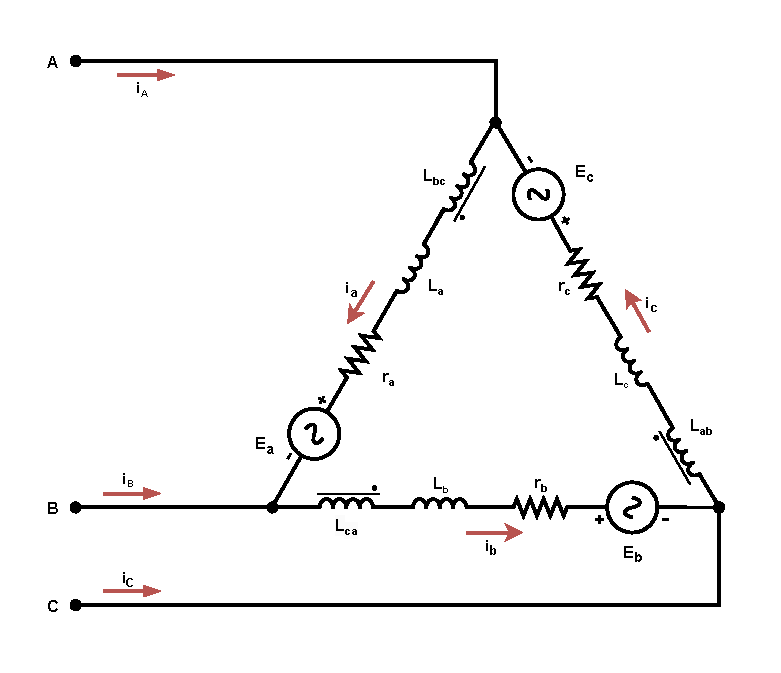
\includegraphics[width=0.6\textwidth]{Figures/Delta_model.pdf}
	\caption[Delta-wound \gls{pmsm}.]{Delta-wound \gls{pmsm}}
	\label{fig:delta_model}%chktex 24
\end{figure}
The expanded form results in~\Cref{eq:voltage_balance}.

\begin{equation}
	\mathbf{u_{abc}}
	=
	\mathbf{R_{abc}}
	\mathbf{i_{abc}}
	+
	% \begin{bmatrix}
	% 	L_{a}  & M_{ab} & M_{ac} \\
	% 	M_{ba} & L_{b}  & M_{bc} \\
	% 	M_{ca} & M_{cb} & L_{c}  \\
	% \end{bmatrix}
	\mathbf{L_{abc}}
	\frac{d\mathbf{i_{abc}}}{dt}
	+
	\frac{d\mathbf{L_{abc}}}{dt}  \mathbf{i_{abc}}
	+\mathbf{E_{abc}}
	\label{eq:voltage_balance}%chktex 24
\end{equation}


% \begin{equation}
% 	E_a + E_b + E_c + r(i_a + i_b + i_c) + (\mathbf{L} - 2\mathbf{M})\left( \frac{di_a}{dt} + \frac{di_b}{dt} + \frac{di_c}{dt}\right) = 0%chktex 7
% \end{equation}
Note that the inductances are not constant, but they change regarding the rotor electrical position $\theta_e$. This variation exists because the selected machine has a spoke magnet arrangement on the rotor, thus creating magnetic paths with different reluctances depending on the rotor angle. According to~\citet{Marques:Dinamica_das_maquinas_eletricas:2002}, this variation is a sum of even harmonics of a cosine function, but usually, it is enough to consider up to the second one, resulting in the inductance matrix shown in~\Cref{eq:phase_inductances}, where $L_{x_1}$,$L_{x_2}$,$M_{xy_1}$, and $M_{xy_2}$ are constants and define the coefficients for the self inductances and the mutual inductances.

\begin{equation}
	\mathbf{L_{abc}} =
	\begin{bmatrix}
		L_{a_1} + L_{a_2} \cos{ \left(2 \theta_e\right)}                    & M_{ab_1} + M_{ab_2} \cos{ \left(2 \theta_e + \frac{4\pi}{3}\right)} & M_{ac_1} + M_{ac_2} \cos{ \left(2 \theta_e - \frac{4\pi}{3}\right)} \\
		M_{ba_1} + M_{ba_2} \cos{ \left(2 \theta_e + \frac{4\pi}{3}\right)} & L_{b_1} + L_{b_2} \cos{ \left(2 \theta_e - \frac{4\pi}{3}\right)}   & M_{bc_1} + M_{bc_2} \cos{ \left(2 \theta_e\right)}                  \\
		M_{ca_1} + M_{ca_2} \cos{ \left(2 \theta_e - \frac{4\pi}{3}\right)} & M_{cb_1} + M_{cb_2} \cos{ \left(2 \theta_e\right)}                  & L_{c_1} + L_{c_2} \cos{ \left(2 \theta_e + \frac{4\pi}{3}\right)}   \\
	\end{bmatrix}
	\label{eq:phase_inductances}
\end{equation}

Is important to explain that the~\Cref{eq:phase_inductances} is derived assuming the 3 phases are separated by $120$ electrical degrees and that the windings have a sinusoidal magnetomotive force distribution.

For comprehensive understanding, the self inductances $L_x$ and the mutual inductances $L_{xy}$ depicted in \Cref{fig:delta_model} are as defined in \Cref{eq:induc_figure}.

\begin{subequations}
	\noindent
	\begin{minipage}{.485\linewidth}
		\begin{equation}
			L_{ab} = M_{ab_1} + M_{ab_2} \cos{ \left(2 \theta_e + \frac{4\pi}{3}\right)}
		\end{equation}
	\end{minipage}
	\begin{minipage}{.485\linewidth}
		\begin{equation}
			L_{ac} = M_{ac_1} + M_{ac_2} \cos{ \left(2 \theta_e - \frac{4\pi}{3}\right)}
		\end{equation}
	\end{minipage}
	\\
	\begin{minipage}{.485\linewidth}
		\begin{equation}
			L_{ba} = M_{ba_1} + M_{ba_2} \cos{ \left(2 \theta_e + \frac{4\pi}{3}\right)}
		\end{equation}
	\end{minipage}
	\begin{minipage}{.485\linewidth}
		\begin{equation}
			L_{bc} = M_{bc_1} + M_{bc_2} \cos{ \left(2 \theta_e\right)}
		\end{equation}
	\end{minipage}
	\\
	\begin{minipage}{.485\linewidth}
		\begin{equation}
			L_{ca} = M_{ca_1} + M_{ca_2} \cos{ \left(2 \theta_e - \frac{4\pi}{3}\right)}
		\end{equation}
	\end{minipage}
	\begin{minipage}{.485\linewidth}
		\begin{equation}
			L_{cb} = M_{cb_1} + M_{cb_2} \cos{ \left(2 \theta_e\right)}
		\end{equation}
	\end{minipage}
	\\
	\begin{minipage}{.485\linewidth}
		\begin{equation}
			L_{a} = L_{a_1} + L_{a_2} \cos{ \left(2 \theta_e\right)}
		\end{equation}
	\end{minipage}
	\begin{minipage}{.485\linewidth}
		\begin{equation}
			L_{b} = L_{b_1} + L_{b_2} \cos{ \left(2 \theta_e\right)}
		\end{equation}
	\end{minipage}
	\\
	\begin{minipage}{.95\linewidth}
		\begin{equation}
			L_{c} = L_{c_1} + L_{c_2} \cos{ \left(2 \theta_e\right)}
		\end{equation}
	\end{minipage}
	\label{eq:induc_figure}
\end{subequations}
%%%%%%%%%%%%%%%%%%%%%%%%%%%%%%%%%%%%%%%%%%%%%%%%%%
\subsection{dq0 Transformation}
\vfill
To simplify the mathematical models, some transformations were proposed. The most common is the dq0 transformation, which is a combination of the Concordia and the Blondel-Park transformations. The Concordia transformation converts a three-phase system into an equivalent two-phase system, where the two phases are orthogonal to each other, they are called $\alpha$ and $\beta$ components. This transformation has two main versions, the amplitude invariant, and the power invariant. The power invariant version, initially presented in \Cref{eq:concordia}, is shown again in \Cref{eq:concordia1} for easier reference.

The Blondel-Park transformation is a rotating referential transformation, where the referential is synchronous with the rotor position. The transformation matrix is shown in \Cref{eq:blondel_park}. Note that throughout this work the alignment of the transformation is always the $d$ component with the phase $a$. The dq0 transformation is a combination of the Concordia transformation, and the Park referential change, it produces a biphasic equivalent system with a synchronous rotating referential. The transformation matrix is shown in \Cref{eq:dq0}.

\begin{subequations}
	% \noindent
	\begin{minipage}{.4\linewidth}
		\begin{equation}
			\mathbf{Co} = \sqrt{\frac{2}{3}}
			\begin{bmatrix}
				1            & 0                   & \frac{1}{\sqrt{2}} \\
				-\frac{1}{2} & \frac{\sqrt{3}}{2}  & \frac{1}{\sqrt{2}} \\
				-\frac{1}{2} & -\frac{\sqrt{3}}{2} & \frac{1}{\sqrt{2}} \\
			\end{bmatrix}
			\label{eq:concordia1}
		\end{equation}
	\end{minipage}
	\begin{minipage}{.485\linewidth}
		\begin{equation}
			\mathbf{Bl}_{(\theta_e)} = 	\begin{bmatrix}
				\cos{\left(\theta_e\right)} & -\sin{\left(\theta_e\right)} & 0 \\
				\sin{\left(\theta_e\right)} & \cos{\left(\theta_e\right)}  & 0 \\
				0                           & 0                            & 1 \\
			\end{bmatrix}
			\label{eq:blondel_park}
		\end{equation}
	\end{minipage}
\end{subequations}
\begin{equation}
	\mathbf{T}_{(\theta_e)} = \mathbf{Co} \; \mathbf{Bl}_{(\theta_e)}
	=
	\sqrt{\frac{2}{3}}
	\begin{bmatrix}
		\cos{\left(\theta_e\right)}                & -\sin{\left(\theta_e\right)}                & \frac{1}{\sqrt{2}} \\
		\cos{\left(\theta_e-\frac{2\pi}{3}\right)} & -\sin{\left(\theta_e-\frac{2\pi}{3}\right)} & \frac{1}{\sqrt{2}} \\
		\cos{\left(\theta_e-\frac{4\pi}{3}\right)} & -\sin{\left(\theta_e-\frac{4\pi}{3}\right)} & \frac{1}{\sqrt{2}} \\
	\end{bmatrix}
	\label{eq:dq0}
\end{equation}

The power invariant transformation has the advantage of being an orthogonal matrix, thus $\mathbf{T}^{-1} = \mathbf{T}^T$.\\
If the amplitude invariant form is used, as in \Cref{eq:blondel_park_amplitude_invariant}, then orthogonality is lost.

\begin{subequations}
	% \begin{minipage}{.45\linewidth}
	\begin{equation}
		\mathbf{T}^*_{(\theta_e)} =
		\begin{bmatrix}
			\cos{\left(\theta_e\right)}                & -\sin{\left(\theta_e\right)}                & 1 \\
			\cos{\left(\theta_e-\frac{2\pi}{3}\right)} & -\sin{\left(\theta_e-\frac{2\pi}{3}\right)} & 1 \\
			\cos{\left(\theta_e-\frac{4\pi}{3}\right)} & -\sin{\left(\theta_e-\frac{4\pi}{3}\right)} & 1 \\
		\end{bmatrix}
	\end{equation}
	% \end{minipage}%
	% \begin{minipage}{.55\linewidth}
	\begin{equation}
		{\mathbf{T}^*_{(\theta_e)}}^{-1} = \frac{2}{3}
		\begin{bmatrix}
			\cos{\left(\theta_e\right)}  & \cos{\left(\theta_e-\frac{2\pi}{3}\right)}  & \cos{\left(\theta_e-\frac{4\pi}{3}\right)}  \\
			-\sin{\left(\theta_e\right)} & -\sin{\left(\theta_e-\frac{2\pi}{3}\right)} & -\sin{\left(\theta_e-\frac{4\pi}{3}\right)} \\
			\frac{1}{2}                  & \frac{1}{2}                                 & \frac{1}{2}                                 \\
		\end{bmatrix}
	\end{equation}
	\label{eq:blondel_park_amplitude_invariant}%chktex 24
	% \end{minipage}%
\end{subequations}

Applying the power invariant transformation to the abc variables results in \Cref{eq:variables_dq0}.

\begin{subequations}
	\noindent
	\begin{minipage}{.5\linewidth}
		\begin{equation}
			\mathbf{R_{dq0}} = \mathbf{T}^T_{(\theta_e)} \mathbf{R_{abc}}\mathbf{T}_{(\theta_e)}
		\end{equation}
	\end{minipage}%
	\begin{minipage}{.5\linewidth}
		\begin{equation}
			\mathbf{L_{dq0}} = \mathbf{T}^T_{(\theta_e)} \mathbf{L_{abc}}\mathbf{T}_{(\theta_e)}
		\end{equation}
	\end{minipage}%
	\\
	\begin{minipage}{.33\linewidth}
		\begin{equation}
			\mathbf{i_{abc}} = \mathbf{T}_{(\theta_e)} \mathbf{i_{dq0}}
		\end{equation}
	\end{minipage}%
	\begin{minipage}{.33\linewidth}
		\begin{equation}
			\mathbf{u_{dq0}} = \mathbf{T}^T_{(\theta_e)} \mathbf{u_{abc}}
		\end{equation}
	\end{minipage}%
	\begin{minipage}{.33\linewidth}
		\begin{equation}
			\pmb{\psi_{abc}} = \mathbf{T}_{(\theta_e)} \pmb{\psi_{dq0}}
		\end{equation}
	\end{minipage}%
	\label{eq:variables_dq0}
\end{subequations}

% Or, using the amplitude invariant form:

% \begin{subequations}
% 	\noindent
% 	\begin{minipage}{.5\linewidth}
% 		\begin{equation}
% 			\mathbf{R_{dq0}} = {\mathbf{T}^*_{(\theta_e)}}^{-1} \mathbf{R_{abc}}\mathbf{T}^*_{(\theta_e)}
% 		\end{equation}
% 	\end{minipage}%
% 	\begin{minipage}{.5\linewidth}
% 		\begin{equation}
% 			\mathbf{L_{dq0}} ={\mathbf{T}^*_{(\theta_e)}}^{-1} \mathbf{L_{abc}}\mathbf{T}^*_{(\theta_e)}
% 		\end{equation}
% 	\end{minipage}%
% 	\\
% 	\begin{minipage}{.33\linewidth}
% 		\begin{equation}
% 			\mathbf{i_{abc}} = \mathbf{T}^*_{(\theta_e)} \mathbf{i_{dq0}}
% 		\end{equation}
% 	\end{minipage}%
% 	\begin{minipage}{.33\linewidth}
% 		\begin{equation}
% 			\mathbf{u_{dq0}} = {\mathbf{T}^*_{(\theta_e)}}^{-1} \mathbf{u_{abc}}
% 		\end{equation}
% 	\end{minipage}%
% 	\begin{minipage}{.33\linewidth}
% 		\begin{equation}
% 			\pmb{\psi_{abc}} = \mathbf{T}^*_{(\theta_e)} \pmb{\psi_{dq0}}
% 		\end{equation}
% 	\end{minipage}%
% 	\label{eq:variables_dq0_amplitude}
% \end{subequations}


%%%%%%%%%%%%%%%%%%%%%%%%%%%%%%%%%%%%%%%%%%%%%%%%%%
\subsection{PMSM in dq0 coordinates}

Assuming the three phases are well balanced and using the dq0 transformation (power invariant form) to transform the model into a two-phase system with a rotating referential, new resistance and inductance matrices can be computed to this new referential. The new matrices are shown in \Cref{eq:inductance_and_resistance_dqd0}, with the subscripts $_d$, $_q$,$_0$, denoting the direct axis, the quadrature axis, and the zero-sequence axis, respectively. The transformation of the matrices is detailed in~\citet{Marques:Dinamica_das_maquinas_eletricas:2002}.

\vspace{0.5cm}
\begin{subequations}
	\begin{minipage}{.53\linewidth}
		\begin{equation}
            \mathbf{R_{dq0}} =
            \begin{bmatrix}
                r_a & 0   & 0   \\
                0   & r_b & 0   \\
                0   & 0   & r_c \\
            \end{bmatrix} =
            \begin{bmatrix}
                r & 0 & 0 \\
                0 & r & 0 \\
                0 & 0 & r \\
            \end{bmatrix}
		\end{equation}
	\end{minipage}%
	\begin{minipage}{.43\linewidth}
		\begin{equation}
            \mathbf{L_{dq0}} =
            \begin{bmatrix}
                L_d & 0   & 0   \\
                0   & L_q & 0   \\
                0   & 0   & L_0 \\
            \end{bmatrix}
		\end{equation}
    \end{minipage}
	\label{eq:inductance_and_resistance_dqd0}
\end{subequations}
\vspace{0.5cm}

Starting with \Cref{eq:flx_voltage_balance} and replacing the currents and flux linkages by their dq0 components results in \Cref{eq:voltage_balance_dq0_intermediary}.

\begin{equation}
	\begin{aligned}
		\mathbf{u_{abc}}
		=
		\mathbf{R_{abc}}
		\mathbf{T}_{(\theta_e)} \mathbf{i_{dq0}}
		+
		\frac{d\left(\mathbf{T}_{(\theta_e)} \pmb{\psi_{dq0}}\right)}{dt}
		\\
		=
		\mathbf{R_{abc}}
		\mathbf{T}_{(\theta_e)} \mathbf{i_{dq0}}
		+\dot{\theta}_e\frac{d\mathbf{T}_{(\theta_e)}}{d\theta_e}\pmb{\psi_{dq0}}
		+\mathbf{T}_{(\theta_e)}\frac{d \pmb{\psi_{dq0}}}{dt}
	\end{aligned}
	\label{eq:voltage_balance_dq0_intermediary}
\end{equation}
Replacing $\dot{\theta}_e$ with $\omega_e$, and multiplying $\mathbf{T}^T_{(\theta_e)}$ to the left yelds \Cref{eq:voltage_balance_dq0_intermediary2}.
\begin{equation}
	\begin{aligned}
		\mathbf{u_{dq0}}
		=
		\mathbf{R_{dq0}}\mathbf{i_{dq0}}
		+\mathbf{T}^T_{(\theta_e)}\omega_e\frac{d\mathbf{T}_{(\theta_e)}}{d\theta_e}\pmb{\psi_{dq0}}
		+\mathbf{T}^T_{(\theta_e)}\mathbf{T}_{(\theta_e)}\frac{d \pmb{\psi_{dq0}}}{dt}
	\end{aligned}
	\label{eq:voltage_balance_dq0_intermediary2}
\end{equation}
As the transformation matrix is orthogonal, it can be further simplified, as in \Cref{eq:voltage_balance_dq0_intermediary3}.
\begin{equation}
	\begin{aligned}
		\mathbf{u_{dq0}}
		=
		\mathbf{R_{dq0}}\mathbf{i_{dq0}}
		+\omega_e\mathbf{T}^T_{(\theta_e)}\frac{d\mathbf{T}_{(\theta_e)}}{d\theta_e}\pmb{\psi_{dq0}}
		+\frac{d \pmb{\psi_{dq0}}}{dt}
	\end{aligned}
	\label{eq:voltage_balance_dq0_intermediary3}
\end{equation}
Lastly, calculate the derivative of the transformation matrix, as in \Cref{eq:transformation_derivative_intermediary,eq:transformation_derivative}.
\begin{equation}
	\label{eq:transformation_derivative_intermediary}
	\mathbf{T}^T_{(\theta_e)}\frac{d\mathbf{T}_{(\theta_e)}}{d\theta_e} = 	\frac{2}{3}
	\begin{bmatrix}
		\cos{\left(\theta_e\right)}  & \cos{\left(\theta_e-\frac{2\pi}{3}\right)}  & \cos{\left(\theta_e-\frac{4\pi}{3}\right)}  \\
		-\sin{\left(\theta_e\right)} & -\sin{\left(\theta_e-\frac{2\pi}{3}\right)} & -\sin{\left(\theta_e-\frac{4\pi}{3}\right)} \\
		\frac{1}{\sqrt{2}}           & \frac{1}{\sqrt{2}}                          & \frac{1}{\sqrt{2}}                          \\
	\end{bmatrix}
	\begin{bmatrix}
		-\sin{\left(\theta_e\right)}                & -\cos{\left(\theta_e\right)}                & 0 \\
		-\sin{\left(\theta_e-\frac{2\pi}{3}\right)} & -\cos{\left(\theta_e-\frac{2\pi}{3}\right)} & 0 \\
		-\sin{\left(\theta_e-\frac{4\pi}{3}\right)} & -\cos{\left(\theta_e-\frac{4\pi}{3}\right)} & 0 \\
	\end{bmatrix}
\end{equation}
\begin{equation}
	\label{eq:transformation_derivative}
	\mathbf{T}^T_{(\theta_e)}\frac{d\mathbf{T}_{(\theta_e)}}{d\theta_e} =
	\begin{bmatrix}
		0 & -1 & 0 \\
		1 & 0  & 0 \\
		0 & 0  & 0 \\
	\end{bmatrix}
\end{equation}
Thus, the \gls{pmsm} model in the dq0 frame is presented in \Cref{eq:flx_voltage_balance_dq0}. This approach can be used for the amplitude invariant transformation and will result in the same form of equation (\Cref{chapter:appendixdq0_amplitude}), but the equation will be scaled by a factor of $\sqrt{\frac{3}{2}}$ in the d and q axis, while the zero axis can give different results.
\begin{equation}
	\mathbf{u_{dq0}}
	=
	\mathbf{R_{dq0}}\mathbf{i_{dq0}}
	+\omega_e	\begin{bmatrix}
		0 & -1 & 0 \\
		1 & 0  & 0 \\
		0 & 0  & 0 \\
	\end{bmatrix}
	\pmb{\psi_{dq0}}
	+\frac{d \pmb{\psi_{dq0}}}{dt}
	\label{eq:flx_voltage_balance_dq0}
\end{equation}

Is worth noticing that because this is a delta wound machine, the sum of the phase currents is not necessarily zero, and as such, it is mathematically possible to have a circulating current through the phases~\cite{Pramod:circulating_currents_delta_winding:2023}, thus the zero-sequence component is not directly zero as in a Y wound device. For such currents to exist, an external exciting winding, a relevant non-considered inductance harmonic, or an imbalance through the phases is necessary. Even when those currents are present, they are usually dependent on the rotor position, and cannot be controlled with the standard 3-terminal connection,
% \textbf{REFERENCE HERE}. Some studies have shown that the zero-sequence current component is relatively small compared to the direct and quadrature ones \textbf{REFERENCE HERE}, and
thus for the sake of simplicity, they are discarded throughout this work, which gives \Cref{eq:motor_blondel_park}.
\begin{subequations}
	\begin{equation}
		u_d = r i_d+\frac{d\psi_d}{dt} - \omega_e \psi_q\\
		\label{eq:motor_blondel_park_d} %chktex 24
	\end{equation}
	\begin{equation}
		u_q = r i_q+\frac{d\psi_q}{dt} + \omega_e \psi_d\\
		\label{eq:motor_blondel_park_q} %chktex 24
	\end{equation}
	\begin{equation}
		T_e = p(\psi_d i_q - \psi_q i_d)\\
	\end{equation}
	\begin{equation}
		\frac{d\omega_e}{dt} = \frac{T_e-T_{load} - T_{loss}}{J}\\
	\end{equation}
	\begin{equation}
		\frac{d\theta_e}{dt} = \omega_e
	\end{equation}
	\label{eq:motor_blondel_park} %chktex 24
\end{subequations}

Here $\omega_e$ is the rotor electrical rotational velocity, $p$ is the number of pole pairs, $J$ is the rotor rotational inertia, while $T_e$ is the electromagnetic torque, $T_{load}$ is the reaction torque of the load attached to the motor, and $T_{loss}$ is a torque equivalent to the losses on the motor (such as iron or friction losses).



If $\psi$ is assumed to be of form $\psi = i_x L_x + \psi_{PM_x}$ where the inductance only varies with the current and the permanent magnets flux ($\psi_{PM_x}$) is defined as constant and affecting only the direct axis ($\psi_{PM_q} = 0$), \Cref{eq:motor_blondel_park_d,eq:motor_blondel_park_q} result in \Cref{eq:motor_with_inductances}.

\begin{subequations}
	\begin{equation}
		% \left\{
		% \begin{aligned}
		u_d = r i_d+\frac{d i_d}{dt}\left(L_d + i_d\frac{d L_d}{di_d}\right) - \omega_e L_q i_q                \\
	\end{equation}
	\begin{equation}
		u_q = r i_q+ \frac{d i_q}{dt} \left(L_q + i_q\frac{d L_q}{di_q}\right) + \omega_e (L_d i_d +\psi_{PM}) \\
		% T_e  = p\, i_q(( L_d - L_q)i_d + \psi_{PM})                                                              \\ %= p( (L_d i_d + \psi_{PM}) i_q - L_q i_q i_d)\\
		% \frac{d\omega_e}{dt} = \frac{T_e-T_{load} - T_{loss}}{J}                                                 \\
		% \frac{d\theta_e}{dt} = \omega_e
		% \end{aligned}
		% \right.
	\end{equation}
	\label{eq:motor_with_inductances}
\end{subequations}
Note that in \Cref{eq:motor_with_inductances} the cross-magnetization effect is not accounted for, but the saturation is included in the inductance variation~\cite{Ohm:saturation_inductance:2000}.
If the inductance derivative is small when compared with the other terms, it can be further simplified to \Cref{eq:motor_with_inductances_no_derivative}.
\begin{subequations}
	\begin{equation}
		% \left\{
		% \begin{aligned}
		u_d = r i_d+L_d\frac{d i_d}{dt} - \omega_e L_q i_q              \\
	\end{equation}
	\begin{equation}
		u_q = r i_q+L_q\frac{d i_q}{dt} + \omega_e (L_d i_d +\psi_{PM})
	\end{equation}
	\begin{equation}
		T_e  = p\, i_q(( L_d - L_q)i_d + \psi_{PM})                       \\ %= p( (L_d i_d + \psi_{PM}) i_q - L_q i_q i_d)
	\end{equation}
	\begin{equation}
		\frac{d\omega_e}{dt} = \frac{T_e-T_{load} - T_{loss}}{J}
	\end{equation}
	\begin{equation}
		\frac{d\theta_e}{dt} = \omega_e
		% \end{aligned}
		% \right.
	\end{equation}
	\label{eq:motor_with_inductances_no_derivative}
\end{subequations}

Lastly, for the sake of completeness, if the amplitude invariant dq0 transformation is used, the currents need to be multiplied by a factor of $\sqrt{\frac{3}{2}}$ in the torque equation to have a power conservative output, resulting in~\Cref{eq:torque_amplitude_invariant}. The $\sqrt{\frac{2}{3}}$ next to the $\psi_{PM}$ is just a reminder that the flux linkage value has a different value depending on the dq0 transformation used.
\begin{equation}
	T_e  = 1.5p\, i_q(( L_d - L_q)i_d + \sqrt{\frac{2}{3}}\psi_{PM})
	\label{eq:torque_amplitude_invariant}
\end{equation}
%%%%%%%%%%%%%%%%%%%%%%%%%%%%%%%%%%%%%%%%%%%%%%%%
\subsection{Discretization of the PMSM model}
\vfill
An approximation of the differential equations is needed to discretize the equations to be able to use the model in a discrete time control system. Two usual solutions are the Backward and the Forward Euler methods. Although simpler to compute, the Forward Euler method is prone to instabilities especially in fast systems such as power converters, in contrast with the Backward alternative that is unconditionally stable. Due to this consideration, the Euler Backward technique will be prioritized.

From \Cref{eq:motor_with_inductances_no_derivative}, knowing that the currents and voltages vary with time and that the inductances are dependant on the currents the derivatives are isolated, as shown in \Cref{eq:model_derivatives}.
\begin{subequations}
	\begin{equation}
	\frac{d i_d}{dt} = \frac{u_d - r i_d + \omega_e L_q i_q}{L_d}
	\end{equation}
	\begin{equation}
	\frac{d i_q}{dt} = \frac{u_q - r i_q - \omega_e (L_d i_d +\psi_{PM})}{L_q}
	\end{equation}
	\begin{equation}
		T_e  = p\, i_q(( L_d - L_q)i_d + \psi_{PM})
	\end{equation}
	\begin{equation}
	\frac{d\omega_e}{dt} = \frac{T_e-T_{load} - T_{loss}}{J}
	\end{equation}
	\begin{equation}
	\frac{d\theta_e}{dt} = \omega_e
	\end{equation}
	\label{eq:model_derivatives}
\end{subequations}
 
Then it is possible to discretize the system with $h$ as the sampling time, and $t = kh$. As the Backward Euler method is desired, the derivatives are approximated by \Cref{eq:backward_euler_example}, resulting in \Cref{eq:motor_with_inductances_discrete}

\begin{equation}
    \frac{dy}{dt} = \frac{y(k+1) - y(k)}{h}
	\label{eq:backward_euler_example}
\end{equation}

\begin{equation}
	\left\{
	\begin{aligned}
		\frac{i_{d(k+1)}-i_{d(k)}}{h} = \frac{u_{d(k+1)} -r i_{d(k+1)} +\omega_{e(k+1)} L_{q(i_q(k+1))} i_{q(k+1)}}{L_{d(i_d(k+1))}}               \\
		\frac{i_{q(k+1)}-i_{q(k)}}{h} = \frac{u_{q(k+1)} -r i_{q(k+1)} - \omega_{e(k+1)} (L_{d(i_d(k+1))} i_{d(k+1)} +\psi_{PM})}{L_{q(i_q(k+1))}} \\
		T_{e(k+1)}  = p\, i_{q(k+1)}(( L_{d(i_d(k+1))} - L_{q(i_q(k+1))})i_{d(k+1)} + \psi_{PM})                                                   \\
		\frac{\omega_{e(k+1)} - \omega_{e(k)}}{h} = \frac{T_{e(k+1)}-T_{load(k+1)} - T_{loss(k+1)}}{J}                                             \\
		\frac{\theta_{e(k+1)} - \theta_{e(k)}}{h} = \omega_{e(k+1)}
	\end{aligned}
	\right.
	\label{eq:motor_with_inductances_discrete}
\end{equation}

This set of equations has an algebraic loop, where the currents in $k+1$ depend on the value of $\omega_{(k+1)}$, that depends on the value of $T_{e(k+1)}$ that is defined by the currents in $k+1$. The same thing happens with the inductances, as they depend on the currents, but the currents define the value of inductance. Those problems are solved by first assuming that the inductance change due to the current change in a time step is small enough so that the inductances can be calculated using the previous time step currents ($ L_{x(i_x(k+1))} \approx L_{x(i_x(k+1))} $). Similarly, the rotor speed is assumed to vary little between iterations, so that $\omega_{(k+1)} \approx \omega_{(k)}$.

With those considerations, and rearranging the equations, the system can be solved iteratively, as shown in \Cref{eq:motor_backward_euler_matrix}.

% \begin{equation}
% 	\left\{
% 	\begin{aligned}
% 		i_{d(k+1)}
% 		= \frac{h(u_{d(k+1)} +\omega_{e(k)} L_{q(i_q(k))} i_{q(k+1)}) + i_{d(k)}L_{d(i_d(k))}}{hr  + L_{d(i_d(k))}}                        \\
% 		i_{q(k+1)} =
% 		\frac{h\left(u_{q(k+1)} - \omega_{e(k)} (L_{d(i_d(k))} i_{d(k+1)} +\psi_{PM})\right) + i_{q(k)} L_{q(i_q(k))}}{hr + L_{q(i_q(k))}} \\
% 		T_{e(k+1)}  = p\, i_{q(k+1)}(( L_{d(i_d(k+1))} - L_{q(i_q(k+1))})i_{d(k+1)} + \psi_{PM})                                           \\
% 		\omega_{e(k+1)} = \omega_{e(k)} + h\left(\frac{T_{e(k+1)}-T_{load(k+1)} - T_{loss(k+1)}}{J}\right)                                 \\
% 		\theta_{e(k+1)} = \theta_{e(k)} + h\omega_{e(k+1)}
% 	\end{aligned}
% 	\right.
% 	\label{eq:motor_backward_euler}
% \end{equation}

% Or, in matrix form, as shown in \Cref{eq:motor_backward_euler_matrix}.
\begin{subequations}
	\begin{equation}
		\begin{aligned}
			\begin{bmatrix}
				i_{d(k+1)} \\
				i_{q(k+1)} \\
			\end{bmatrix}
			=
			\begin{bmatrix}
				1                                                    & -h\frac{\omega_{e(k)}L_{q(i_q(k))}}{hr+L_{d(i_d(k))}} \\
				h\frac{\omega_{e(k)}L_{d(i_d(k))}}{hr+L_{q(i_q(k))}} & 1                                                     \\
			\end{bmatrix}^{-1} \\
			\left(
			\begin{bmatrix}
					\frac{L_{d(i_d(k))}}{hr+L_{d(i_d(k))}} & 0                                      \\
					0                                      & \frac{L_{q(i_q(k))}}{hr+L_{q(i_q(k))}} \\
				\end{bmatrix}
			\begin{bmatrix}
					i_{d(k)} \\
					i_{q(k)} \\
				\end{bmatrix}
			+
			\begin{bmatrix}
					\frac{h}{hr+L_{d(i_d(k))}} & 0                          \\
					0                          & \frac{h}{hr+L_{q(i_q(k))}} \\
				\end{bmatrix}
			\begin{bmatrix}
					u_{d(k+1)} \\
					u_{q(k+1)} \\
				\end{bmatrix}
			+
			\begin{bmatrix}
					0                                                 \\
					-h\frac{\omega_{e(k)}\psi_{PM}}{hr+L_{q(i_q(k))}} \\
				\end{bmatrix}
			\right)
		\end{aligned}
	\end{equation}

	\begin{equation}
		T_{e(k+1)}  = p\, i_{q(k+1)}((L_{d(i_d(k+1))} - L_{q(i_q(k+1))})i_{d(k+1)} + \psi_{PM})
	\end{equation}

	\begin{equation}
		\begin{aligned}
			\begin{bmatrix}
				\omega_{e(k+1)} \\
				\theta_{e(k+1)}
			\end{bmatrix}
			=
			\begin{bmatrix}
				1 & 0 \\
				h & 1
			\end{bmatrix}
			\begin{bmatrix}
				\omega_{e(k)} \\
				\theta_{e(k)}
			\end{bmatrix}
			+
			\frac{T_{e(k+1)}-T_{load(k+1)} - T_{loss(k+1)}}{J}
			\begin{bmatrix}
				h \\
				h^2
			\end{bmatrix}
		\end{aligned}
	\end{equation}
	\label{eq:motor_backward_euler_matrix}
\end{subequations}